\documentclass{article}\usepackage[]{graphicx}\usepackage[]{color}
% maxwidth is the original width if it is less than linewidth
% otherwise use linewidth (to make sure the graphics do not exceed the margin)
\makeatletter
\def\maxwidth{ %
  \ifdim\Gin@nat@width>\linewidth
    \linewidth
  \else
    \Gin@nat@width
  \fi
}
\makeatother

\definecolor{fgcolor}{rgb}{0.345, 0.345, 0.345}
\newcommand{\hlnum}[1]{\textcolor[rgb]{0.686,0.059,0.569}{#1}}%
\newcommand{\hlstr}[1]{\textcolor[rgb]{0.192,0.494,0.8}{#1}}%
\newcommand{\hlcom}[1]{\textcolor[rgb]{0.678,0.584,0.686}{\textit{#1}}}%
\newcommand{\hlopt}[1]{\textcolor[rgb]{0,0,0}{#1}}%
\newcommand{\hlstd}[1]{\textcolor[rgb]{0.345,0.345,0.345}{#1}}%
\newcommand{\hlkwa}[1]{\textcolor[rgb]{0.161,0.373,0.58}{\textbf{#1}}}%
\newcommand{\hlkwb}[1]{\textcolor[rgb]{0.69,0.353,0.396}{#1}}%
\newcommand{\hlkwc}[1]{\textcolor[rgb]{0.333,0.667,0.333}{#1}}%
\newcommand{\hlkwd}[1]{\textcolor[rgb]{0.737,0.353,0.396}{\textbf{#1}}}%
\let\hlipl\hlkwb

\usepackage{framed}
\makeatletter
\newenvironment{kframe}{%
 \def\at@end@of@kframe{}%
 \ifinner\ifhmode%
  \def\at@end@of@kframe{\end{minipage}}%
  \begin{minipage}{\columnwidth}%
 \fi\fi%
 \def\FrameCommand##1{\hskip\@totalleftmargin \hskip-\fboxsep
 \colorbox{shadecolor}{##1}\hskip-\fboxsep
     % There is no \\@totalrightmargin, so:
     \hskip-\linewidth \hskip-\@totalleftmargin \hskip\columnwidth}%
 \MakeFramed {\advance\hsize-\width
   \@totalleftmargin\z@ \linewidth\hsize
   \@setminipage}}%
 {\par\unskip\endMakeFramed%
 \at@end@of@kframe}
\makeatother

\definecolor{shadecolor}{rgb}{.97, .97, .97}
\definecolor{messagecolor}{rgb}{0, 0, 0}
\definecolor{warningcolor}{rgb}{1, 0, 1}
\definecolor{errorcolor}{rgb}{1, 0, 0}
\newenvironment{knitrout}{}{} % an empty environment to be redefined in TeX

\usepackage{alltt}

\usepackage{float}
\usepackage{hyperref}

% Set the margins on the page to not be so large
\addtolength{\oddsidemargin}{-.875in}
\addtolength{\evensidemargin}{-.875in}
\addtolength{\textwidth}{1.75in}
\addtolength{\topmargin}{-.875in}
\addtolength{\textheight}{1.75in}

% Take off page numbering
\pagenumbering{gobble}
\IfFileExists{upquote.sty}{\usepackage{upquote}}{}
\begin{document}

\title{%
6.1.1 - R: Time Series \\
\smallskip
\large Stat 5100: Dr. Bean
}
\date{}

\maketitle

\textbf{Example 1: } Bush and the Price of Gas

\begin{enumerate}
\item \href{http://www.leftbusinessobserver.com/BushNGas.html}{http://www.leftbusinessobserver.com/BushNGas.html}
\item ``... no occupant of the White House has ever seen his popularity so closely tied to the price of gas.''
\item ``There's no precedent for this tight relationship.''
\end{enumerate}

\begin{figure}[h]
\centering
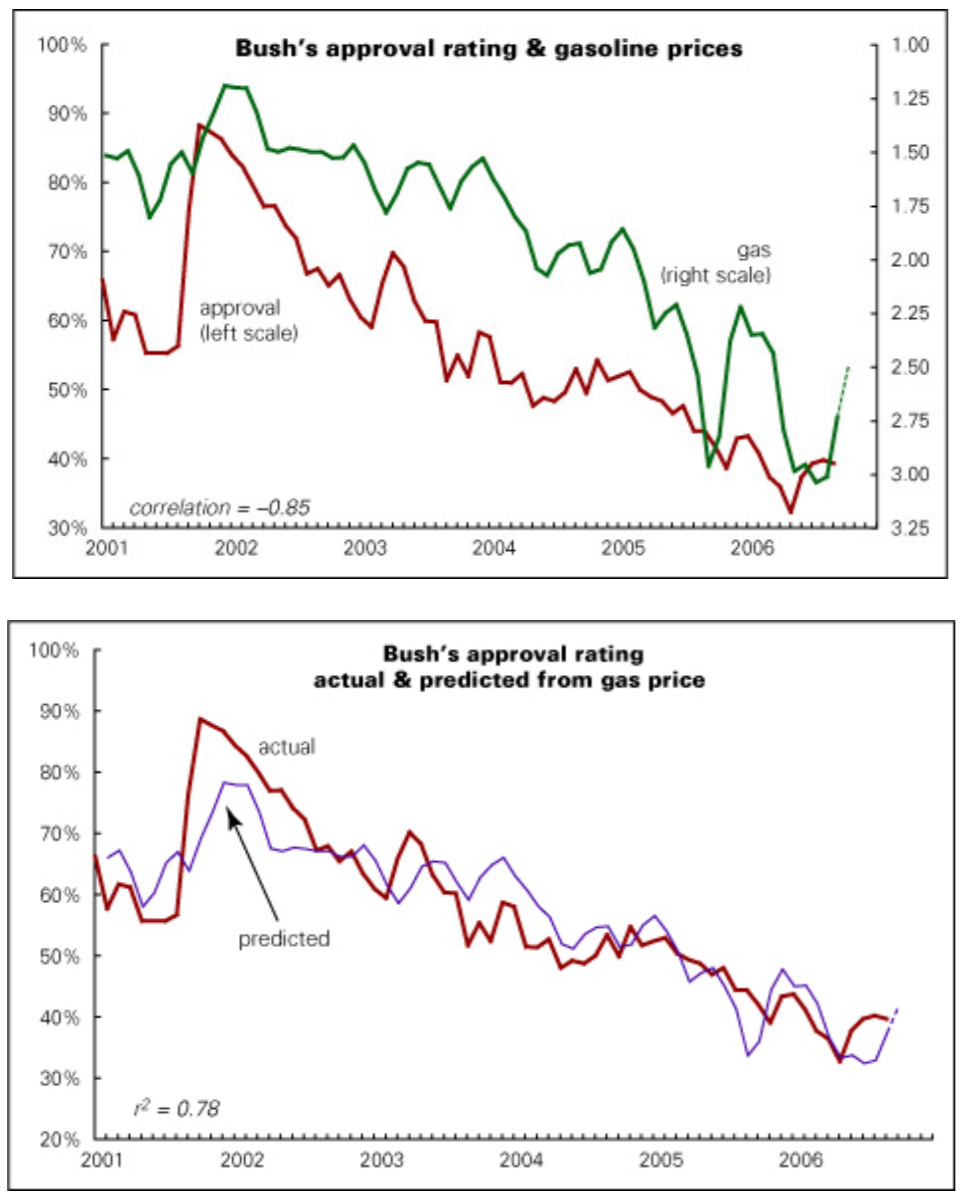
\includegraphics[width = 0.65\textwidth]{../figures/module6/bush_gas_ratings.png}
\end{figure}

But - can we justify a conclusion that gas price significantly affects approval rating? (HW 7 will address this more completely). 

\newpage

\begin{knitrout}
\definecolor{shadecolor}{rgb}{0.969, 0.969, 0.969}\color{fgcolor}\begin{kframe}
\begin{alltt}
\hlkwd{library}\hlstd{(stat5100)}

\hlkwd{data}\hlstd{(bush_gas)}

\hlstd{tlm} \hlkwb{<-} \hlkwd{lm}\hlstd{(rating} \hlopt{~} \hlstd{price,} \hlkwc{data} \hlstd{= bush_gas)}
\hlkwd{summary}\hlstd{(tlm)}
\end{alltt}
\begin{verbatim}
## 
## Call:
## lm(formula = rating ~ price, data = bush_gas)
## 
## Residuals:
##     Min      1Q  Median      3Q     Max 
## -27.423  -4.779  -1.294   3.779  24.099 
## 
## Coefficients:
##             Estimate Std. Error t value Pr(>|t|)    
## (Intercept) 88.80015    2.82573   31.43   <2e-16 ***
## price       -0.18281    0.01242  -14.72   <2e-16 ***
## ---
## Signif. codes:  0 '***' 0.001 '**' 0.01 '*' 0.05 '.' 0.1 ' ' 1
## 
## Residual standard error: 8.77 on 94 degrees of freedom
##   (2 observations deleted due to missingness)
## Multiple R-squared:  0.6975,	Adjusted R-squared:  0.6943 
## F-statistic: 216.7 on 1 and 94 DF,  p-value: < 2.2e-16
\end{verbatim}
\begin{alltt}
\hlkwd{plot}\hlstd{(bush_gas}\hlopt{$}\hlstd{office[}\hlopt{!}\hlkwd{is.na}\hlstd{(bush_gas}\hlopt{$}\hlstd{rating)} \hlopt{& !}\hlkwd{is.na}\hlstd{(bush_gas}\hlopt{$}\hlstd{price)],}
     \hlstd{tlm}\hlopt{$}\hlstd{residuals,} \hlkwc{type} \hlstd{=} \hlstr{"l"}\hlstd{,} \hlkwc{xlab} \hlstd{=} \hlstr{"office"}\hlstd{,} \hlkwc{ylab} \hlstd{=} \hlstr{"residual"}\hlstd{)}
\end{alltt}
\end{kframe}

{\centering 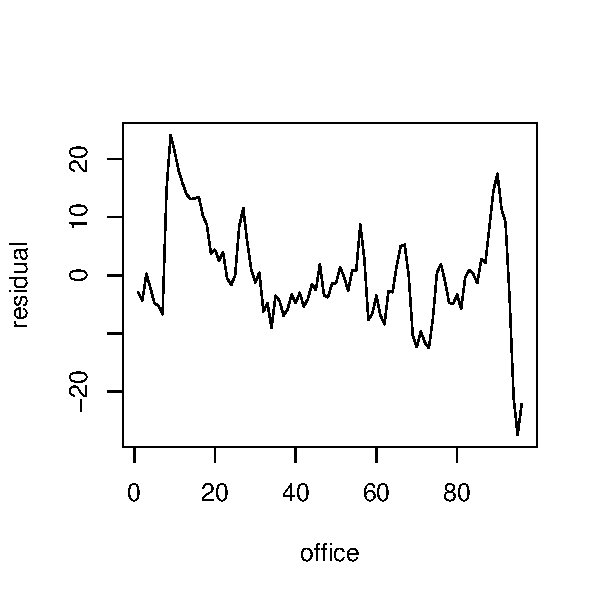
\includegraphics[width=\maxwidth]{figure/unnamed-chunk-1-1} 

}



\end{knitrout}

\newpage

\subsection*{Example 2: General Electric's gross investment (in millions of dollars) for years 1935 - 1954.}

Originally presented in Grunfeld, Y. (1958), "The Determinants of Corporate Investment," Ph.D. dissertation, University of Chicago; discussed in Boot, J.C.G. (1960), "Investment Demand: An Empirical Contribution to the Aggregation Problem," International Economic Review, 1, 3-30. See also Damodar N. Gujarati, Basic Econometrics, Third Edition, 1995, McGraw-Hill, [1995, pp. 522-525].

\begin{knitrout}
\definecolor{shadecolor}{rgb}{0.969, 0.969, 0.969}\color{fgcolor}\begin{kframe}
\begin{alltt}
\hlcom{# Load the GE data}
\hlkwd{data}\hlstd{(ge)}
\hlkwd{head}\hlstd{(ge)}
\end{alltt}
\begin{verbatim}
##   year GEinv
## 1 1935  33.1
## 2 1936  45.0
## 3 1937  77.2
## 4 1938  44.6
## 5 1939  48.1
## 6 1940  74.4
\end{verbatim}
\begin{alltt}
\hlcom{# Create a line plot of GE's gross investment each year.}
\hlkwd{plot}\hlstd{(ge}\hlopt{$}\hlstd{year, ge}\hlopt{$}\hlstd{GEinv,} \hlkwc{main} \hlstd{=} \hlstr{"GE gross investment"}\hlstd{,} \hlkwc{xlab} \hlstd{=} \hlstr{"Year"}\hlstd{,}
     \hlkwc{ylab} \hlstd{=} \hlstr{"GE gross investment (millions)"}\hlstd{,} \hlkwc{type} \hlstd{=} \hlstr{"b"}\hlstd{,} \hlkwc{pch} \hlstd{=} \hlnum{16}\hlstd{)}
\end{alltt}
\end{kframe}

{\centering 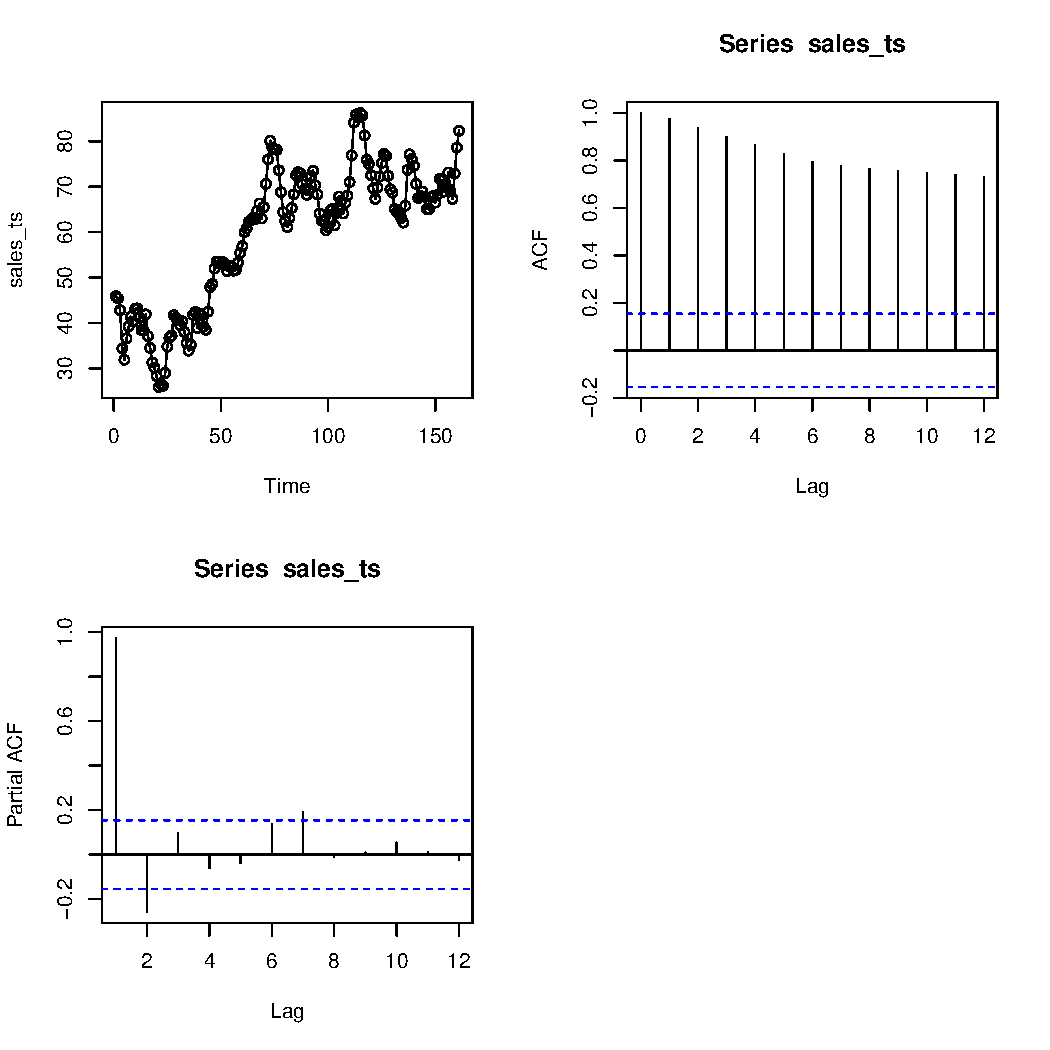
\includegraphics[width=0.6\textwidth]{figure/unnamed-chunk-2-1} 

}



\end{knitrout}

\subsubsection*{(1) Make the data stationary}

\begin{knitrout}
\definecolor{shadecolor}{rgb}{0.969, 0.969, 0.969}\color{fgcolor}\begin{kframe}
\begin{alltt}
\hlcom{# Create a regression model predicting GE investment from year. Next we will}
\hlcom{# examine the residuals (residuals represent the structure after accounting}
\hlcom{# for the time dependence)}
\hlstd{ge_time_lm} \hlkwb{<-} \hlkwd{lm}\hlstd{(GEinv} \hlopt{~} \hlstd{year,} \hlkwc{data} \hlstd{= ge)}

\hlkwd{plot}\hlstd{(ge}\hlopt{$}\hlstd{year, ge_time_lm}\hlopt{$}\hlstd{residuals,} \hlkwc{xlab} \hlstd{=} \hlstr{"Year"}\hlstd{,} \hlkwc{ylab} \hlstd{=} \hlstr{"Residual"}\hlstd{,}
     \hlkwc{main} \hlstd{=} \hlstr{"GE gross investment after accounting for time"}\hlstd{,} \hlkwc{type} \hlstd{=} \hlstr{"b"}\hlstd{,} \hlkwc{pch} \hlstd{=} \hlnum{16}\hlstd{)}
\end{alltt}
\end{kframe}

{\centering 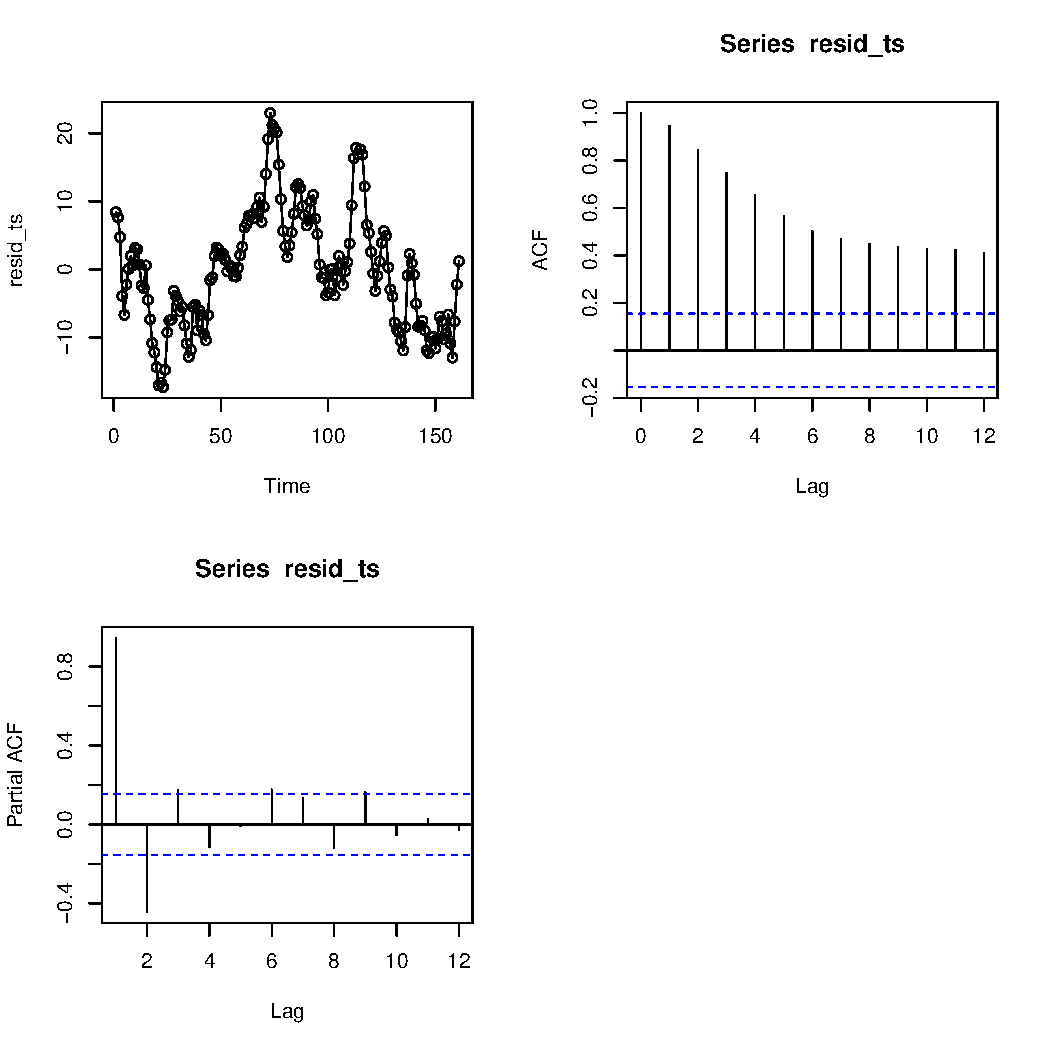
\includegraphics[width=0.6\textwidth]{figure/unnamed-chunk-3-1} 

}


\begin{kframe}\begin{alltt}
\hlcom{# Alternatively, we can make the data stationary after transforming the}
\hlcom{# response variable with a log transformation.}
\hlstd{ge} \hlkwb{<-} \hlkwd{cbind}\hlstd{(ge,} \hlkwc{logGEinv} \hlstd{=} \hlkwd{log}\hlstd{(ge}\hlopt{$}\hlstd{GEinv))}
\hlstd{ge_time_log_lm} \hlkwb{<-} \hlkwd{lm}\hlstd{(logGEinv} \hlopt{~} \hlstd{year,} \hlkwc{data} \hlstd{= ge)}

\hlkwd{plot}\hlstd{(ge}\hlopt{$}\hlstd{year, ge_time_log_lm}\hlopt{$}\hlstd{residuals,} \hlkwc{xlab} \hlstd{=} \hlstr{"Year"}\hlstd{,} \hlkwc{ylab} \hlstd{=} \hlstr{"Residual"}\hlstd{,}
     \hlkwc{main} \hlstd{=} \hlstr{"GE gross investment after accounting for time, using log"}\hlstd{,}
     \hlkwc{type} \hlstd{=} \hlstr{"b"}\hlstd{,} \hlkwc{pch} \hlstd{=} \hlnum{16}\hlstd{)}
\end{alltt}
\end{kframe}

{\centering 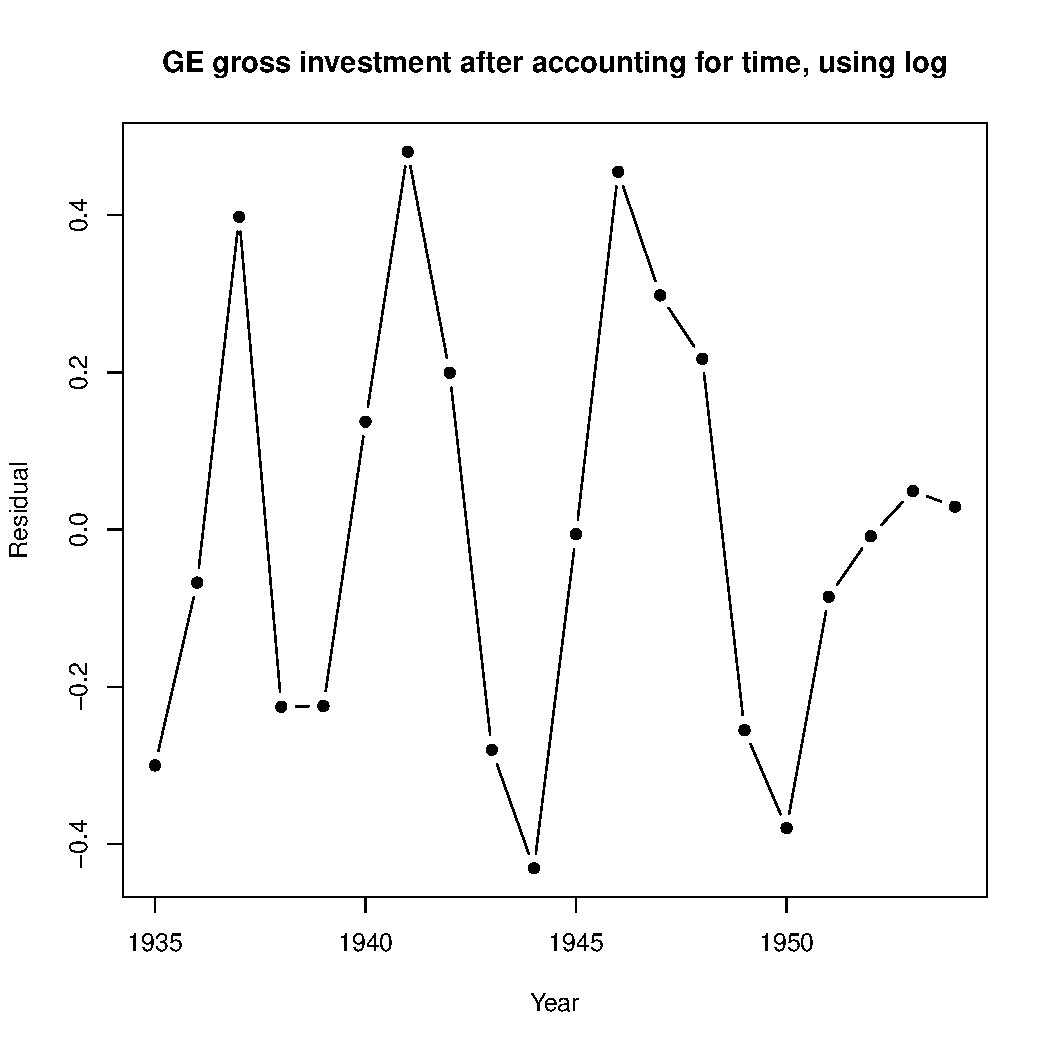
\includegraphics[width=0.6\textwidth]{figure/unnamed-chunk-3-2} 

}



\end{knitrout}

\subsubsection*{(2) Test for independence and (3) investigate potential dependence structures}

\begin{knitrout}
\definecolor{shadecolor}{rgb}{0.969, 0.969, 0.969}\color{fgcolor}\begin{kframe}
\begin{alltt}
\hlcom{# Create a time-series object for our data}
\hlstd{ge_ts} \hlkwb{<-} \hlkwd{ts}\hlstd{(ge_time_log_lm}\hlopt{$}\hlstd{residuals)}

\hlcom{# Sample Autocorrelation Plot (ACF) / Sample Partial Autocorrelation Plots (PACF)}
\hlkwd{par}\hlstd{(}\hlkwc{mfrow} \hlstd{=} \hlkwd{c}\hlstd{(}\hlnum{2}\hlstd{,} \hlnum{1}\hlstd{))}
\hlkwd{acf}\hlstd{(ge_ts,} \hlkwc{lag.max} \hlstd{=} \hlnum{12}\hlstd{)}
\hlkwd{pacf}\hlstd{(ge_ts,} \hlkwc{lag.max} \hlstd{=} \hlnum{12}\hlstd{)}
\end{alltt}
\end{kframe}
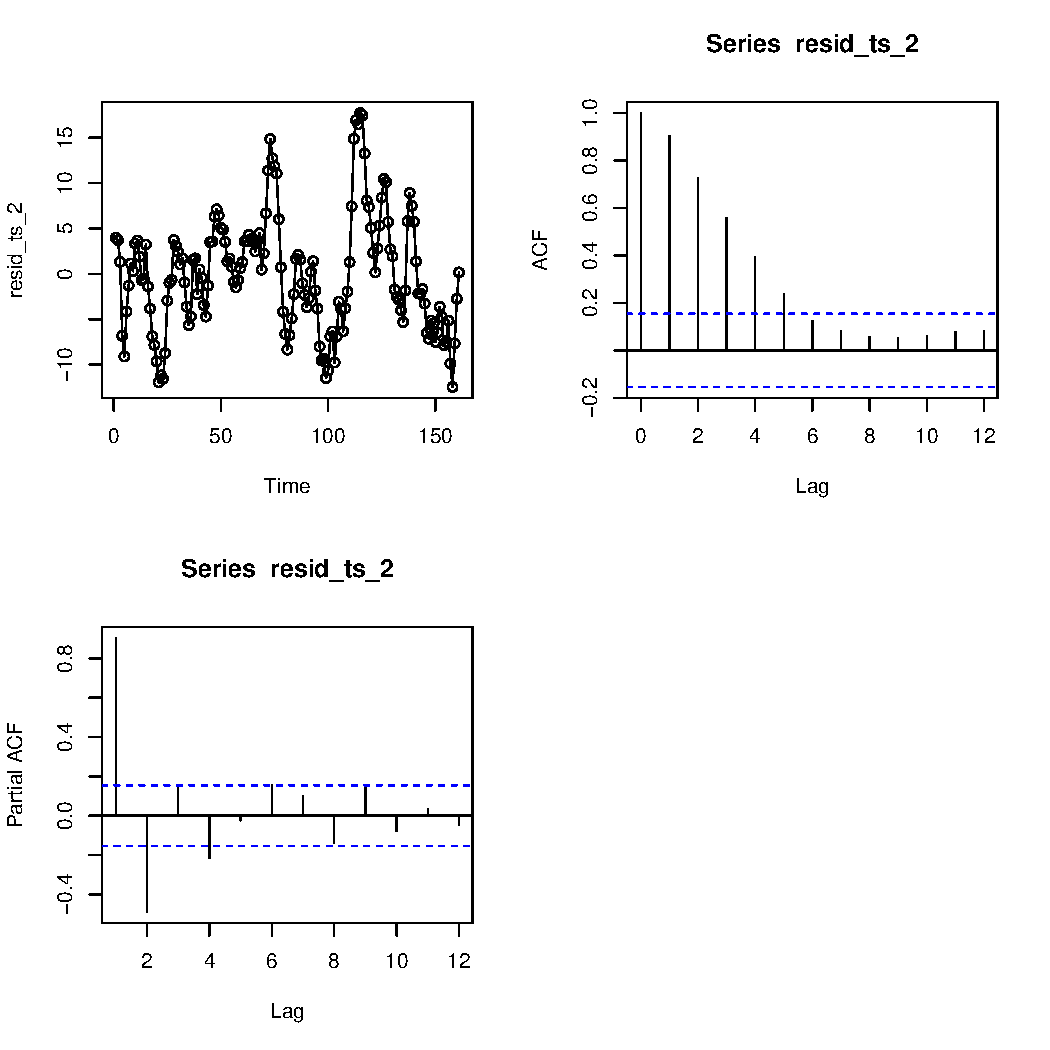
\includegraphics[width=\maxwidth]{figure/unnamed-chunk-4-1} 
\begin{kframe}\begin{alltt}
\hlkwd{par}\hlstd{(}\hlkwc{mfrow} \hlstd{=} \hlkwd{c}\hlstd{(}\hlnum{1}\hlstd{,} \hlnum{1}\hlstd{))}

\hlcom{# Autocorrelation check for white noise}
\hlkwd{Box.test}\hlstd{(ge_ts,} \hlkwc{lag} \hlstd{=} \hlnum{6}\hlstd{,} \hlkwc{type} \hlstd{=} \hlstr{"Ljung"}\hlstd{)}
\end{alltt}
\begin{verbatim}
## 
## 	Box-Ljung test
## 
## data:  ge_ts
## X-squared = 20.425, df = 6, p-value = 0.002326
\end{verbatim}
\begin{alltt}
\hlkwd{Box.test}\hlstd{(ge_ts,} \hlkwc{lag} \hlstd{=} \hlnum{12}\hlstd{,} \hlkwc{type} \hlstd{=} \hlstr{"Ljung"}\hlstd{)}
\end{alltt}
\begin{verbatim}
## 
## 	Box-Ljung test
## 
## data:  ge_ts
## X-squared = 21.331, df = 12, p-value = 0.04574
\end{verbatim}
\end{kframe}
\end{knitrout}

\subsubsection*{(4) Fit a dependence structure and assess model adequacy}
\begin{knitrout}
\definecolor{shadecolor}{rgb}{0.969, 0.969, 0.969}\color{fgcolor}\begin{kframe}
\begin{alltt}
\hlcom{# Fit the original (log transformed) data (not the residuals) and }
\hlcom{# include a drift term which will fit a linear time dependent trend. }
\hlstd{ge_ts} \hlkwb{<-} \hlkwd{ts}\hlstd{(ge}\hlopt{$}\hlstd{logGEinv)}
\hlstd{ge_arima} \hlkwb{<-} \hlstd{forecast}\hlopt{::}\hlkwd{Arima}\hlstd{(ge_ts,} \hlkwc{order} \hlstd{=} \hlkwd{c}\hlstd{(}\hlnum{2}\hlstd{,} \hlnum{0}\hlstd{,} \hlnum{0}\hlstd{),} \hlkwc{include.drift} \hlstd{=} \hlnum{TRUE}\hlstd{)}
\end{alltt}


{\ttfamily\noindent\itshape\color{messagecolor}{\#\# Registered S3 method overwritten by 'quantmod':\\\#\#\ \  method\ \ \ \ \ \ \ \ \ \ \ \ from\\\#\#\ \  as.zoo.data.frame zoo}}\begin{alltt}
\hlkwd{summary}\hlstd{(ge_arima)}
\end{alltt}
\begin{verbatim}
## Series: ge_ts 
## ARIMA(2,0,0) with drift 
## 
## Coefficients:
##          ar1      ar2  intercept   drift
##       0.4871  -0.6507     3.7527  0.0722
## s.e.  0.1668   0.1539     0.0836  0.0071
## 
## sigma^2 estimated as 0.04461:  log likelihood=4.35
## AIC=1.29   AICc=5.58   BIC=6.27
## 
## Training set error measures:
##                        ME      RMSE      MAE       MPE     MAPE      MASE
## Training set -0.004326995 0.1889213 0.143847 -0.321654 3.312231 0.5164973
##                    ACF1
## Training set -0.1389596
\end{verbatim}
\begin{alltt}
\hlcom{# Note that forecast::Arima does not automatically provide p-values. }
\hlcom{# The lmtest package will provide these for you. }
\hlstd{lmtest}\hlopt{::}\hlkwd{coeftest}\hlstd{(ge_arima)}
\end{alltt}
\begin{verbatim}
## 
## z test of coefficients:
## 
##             Estimate Std. Error z value  Pr(>|z|)    
## ar1        0.4870567  0.1667691  2.9205  0.003494 ** 
## ar2       -0.6507009  0.1538594 -4.2292 2.345e-05 ***
## intercept  3.7526822  0.0836412 44.8664 < 2.2e-16 ***
## drift      0.0721521  0.0070884 10.1788 < 2.2e-16 ***
## ---
## Signif. codes:  0 '***' 0.001 '**' 0.01 '*' 0.05 '.' 0.1 ' ' 1
\end{verbatim}
\begin{alltt}
\hlcom{# Create a panel of plots to diagnose the results of the ARIMA predictions}
\hlkwd{par}\hlstd{(}\hlkwc{mfrow} \hlstd{=} \hlkwd{c}\hlstd{(}\hlnum{2}\hlstd{,} \hlnum{1}\hlstd{))}
\hlkwd{acf}\hlstd{(ge_arima}\hlopt{$}\hlstd{residuals,} \hlkwc{lag.max} \hlstd{=} \hlnum{12}\hlstd{)}
\hlkwd{pacf}\hlstd{(ge_arima}\hlopt{$}\hlstd{residuals,} \hlkwc{lag.max} \hlstd{=} \hlnum{12}\hlstd{)}
\end{alltt}
\end{kframe}
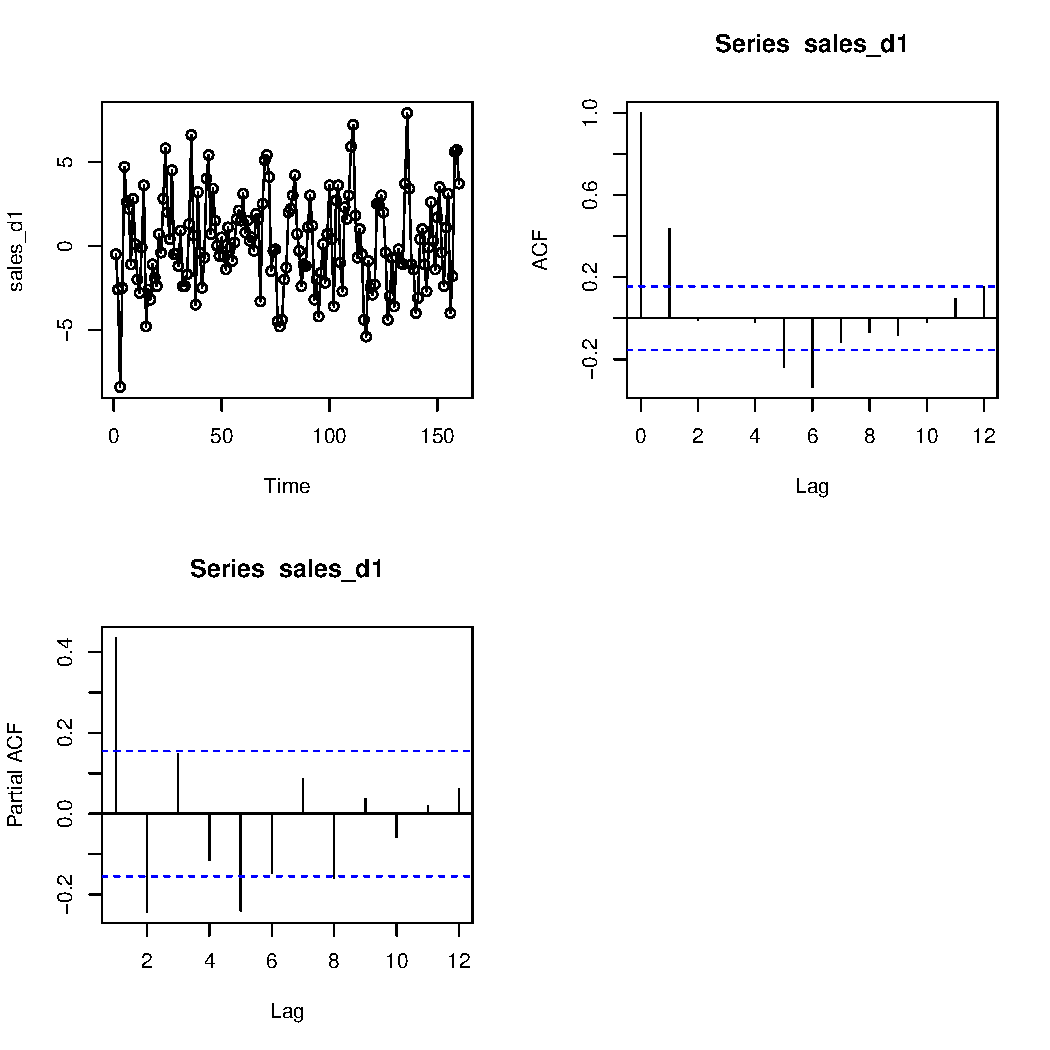
\includegraphics[width=\maxwidth]{figure/unnamed-chunk-5-1} 
\begin{kframe}\begin{alltt}
\hlkwd{par}\hlstd{(}\hlkwc{mfrow} \hlstd{=} \hlkwd{c}\hlstd{(}\hlnum{1}\hlstd{,} \hlnum{1}\hlstd{))}

\hlcom{# Autocorrelation check of residuals}
\hlkwd{Box.test}\hlstd{(ge_arima}\hlopt{$}\hlstd{residuals,} \hlkwc{lag} \hlstd{=} \hlnum{6}\hlstd{,} \hlkwc{type} \hlstd{=} \hlstr{"Ljung"}\hlstd{)}
\end{alltt}
\begin{verbatim}
## 
## 	Box-Ljung test
## 
## data:  ge_arima$residuals
## X-squared = 2.9163, df = 6, p-value = 0.8193
\end{verbatim}
\begin{alltt}
\hlkwd{Box.test}\hlstd{(ge_arima}\hlopt{$}\hlstd{residuals,} \hlkwc{lag} \hlstd{=} \hlnum{12}\hlstd{,} \hlkwc{type} \hlstd{=} \hlstr{"Ljung"}\hlstd{)}
\end{alltt}
\begin{verbatim}
## 
## 	Box-Ljung test
## 
## data:  ge_arima$residuals
## X-squared = 8.2374, df = 12, p-value = 0.7663
\end{verbatim}
\begin{alltt}
\hlkwd{Box.test}\hlstd{(ge_arima}\hlopt{$}\hlstd{residuals,} \hlkwc{lag} \hlstd{=} \hlnum{18}\hlstd{,} \hlkwc{type} \hlstd{=} \hlstr{"Ljung"}\hlstd{)}
\end{alltt}
\begin{verbatim}
## 
## 	Box-Ljung test
## 
## data:  ge_arima$residuals
## X-squared = 12.576, df = 18, p-value = 0.8161
\end{verbatim}
\end{kframe}
\end{knitrout}

\subsubsection*{(5) Forecast}

\begin{knitrout}
\definecolor{shadecolor}{rgb}{0.969, 0.969, 0.969}\color{fgcolor}\begin{kframe}
\begin{alltt}
\hlcom{# 1.645 is the z-score associated with a 90 percent confidence interval}
\hlstd{current} \hlkwb{<-} \hlkwd{data.frame}\hlstd{(}\hlkwc{fit} \hlstd{=} \hlkwd{as.numeric}\hlstd{(ge_arima}\hlopt{$}\hlstd{fitted),}
                      \hlkwc{lower} \hlstd{=} \hlkwd{as.numeric}\hlstd{(ge_arima}\hlopt{$}\hlstd{fitted} \hlopt{-}
                                           \hlnum{1.64}\hlopt{*}\hlkwd{sqrt}\hlstd{(ge_arima}\hlopt{$}\hlstd{sigma2)),}
                      \hlkwc{upper} \hlstd{=} \hlkwd{as.numeric}\hlstd{(ge_arima}\hlopt{$}\hlstd{fitted} \hlopt{+}
                                           \hlnum{1.64}\hlopt{*}\hlkwd{sqrt}\hlstd{(ge_arima}\hlopt{$}\hlstd{sigma2)),}
                      \hlkwc{year} \hlstd{= ge}\hlopt{$}\hlstd{year)}

\hlstd{ahead} \hlkwb{<-} \hlstd{forecast}\hlopt{::}\hlkwd{forecast}\hlstd{(ge_arima,} \hlkwc{h} \hlstd{=} \hlnum{6}\hlstd{,} \hlkwc{level} \hlstd{=} \hlnum{90}\hlstd{)}
\hlstd{ahead} \hlkwb{<-} \hlkwd{data.frame}\hlstd{(}\hlkwc{fit} \hlstd{=} \hlkwd{as.numeric}\hlstd{(ahead}\hlopt{$}\hlstd{mean),}
                    \hlkwc{lower} \hlstd{=} \hlkwd{as.numeric}\hlstd{(ahead}\hlopt{$}\hlstd{lower[,} \hlnum{1}\hlstd{]),}
                    \hlkwc{upper} \hlstd{=} \hlkwd{as.numeric}\hlstd{(ahead}\hlopt{$}\hlstd{upper[ ,}\hlnum{1}\hlstd{]),}
                    \hlkwc{year} \hlstd{= (}\hlkwd{max}\hlstd{(ge}\hlopt{$}\hlstd{year)} \hlopt{+} \hlnum{1}\hlstd{)}\hlopt{:}\hlstd{(}\hlkwd{max}\hlstd{(ge}\hlopt{$}\hlstd{year)} \hlopt{+} \hlnum{6}\hlstd{))}

\hlstd{final} \hlkwb{<-} \hlkwd{rbind}\hlstd{(current, ahead)}


\hlkwd{plot}\hlstd{(final}\hlopt{$}\hlstd{year, final}\hlopt{$}\hlstd{fit,} \hlkwc{col} \hlstd{=} \hlstr{"red"}\hlstd{,} \hlkwc{type} \hlstd{=} \hlstr{"l"}\hlstd{,}
     \hlkwc{xlab} \hlstd{=} \hlstr{"year"}\hlstd{,} \hlkwc{ylab} \hlstd{=} \hlstr{"log of GE gross investment (millions)"}\hlstd{,}
     \hlkwc{ylim} \hlstd{=} \hlkwd{c}\hlstd{(}\hlnum{3.25}\hlstd{,} \hlnum{6.25}\hlstd{),}
     \hlkwc{main} \hlstd{=} \hlstr{"Model Fit: ARIMA(2, 0, 0)"}\hlstd{)}
\hlkwd{lines}\hlstd{(final}\hlopt{$}\hlstd{year, final}\hlopt{$}\hlstd{lower,} \hlkwc{lty} \hlstd{=} \hlnum{2}\hlstd{)}
\hlkwd{lines}\hlstd{(final}\hlopt{$}\hlstd{year, final}\hlopt{$}\hlstd{upper,} \hlkwc{lty} \hlstd{=} \hlnum{2}\hlstd{)}
\hlkwd{lines}\hlstd{(ge}\hlopt{$}\hlstd{year, ge}\hlopt{$}\hlstd{logGEinv,} \hlkwc{lwd} \hlstd{=} \hlnum{2}\hlstd{,} \hlkwc{col} \hlstd{=} \hlstr{"blue"}\hlstd{)}
\hlkwd{legend}\hlstd{(}\hlstr{"topleft"}\hlstd{,} \hlkwc{legend} \hlstd{=} \hlkwd{c}\hlstd{(}\hlstr{"Observed"}\hlstd{,} \hlstr{"Forecast"}\hlstd{,}
                             \hlstr{"Upper CL (90%)"}\hlstd{,}
                             \hlstr{"Lower CL (90%)"}\hlstd{),}
       \hlkwc{lty} \hlstd{=} \hlkwd{c}\hlstd{(}\hlnum{1}\hlstd{,} \hlnum{1}\hlstd{,} \hlnum{2}\hlstd{,} \hlnum{2}\hlstd{),}
       \hlkwc{col} \hlstd{=} \hlkwd{c}\hlstd{(}\hlstr{"blue"}\hlstd{,} \hlstr{"red"}\hlstd{,} \hlstr{"black"}\hlstd{,} \hlstr{"black"}\hlstd{))}
\end{alltt}
\end{kframe}

{\centering 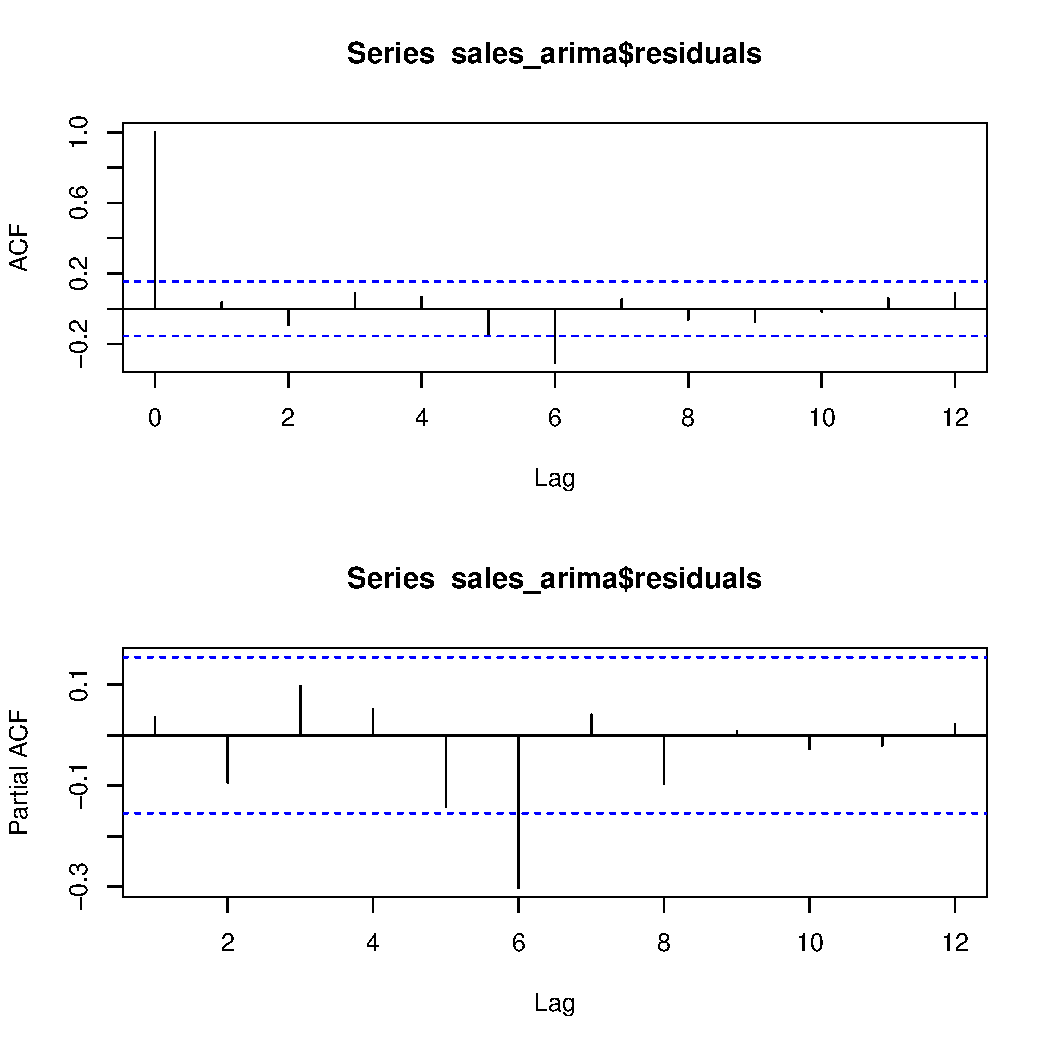
\includegraphics[width=\maxwidth]{figure/unnamed-chunk-6-1} 

}



\end{knitrout}


\subsubsection*{ARMA(1, 1) model (for comparison purposes only)}
\begin{knitrout}
\definecolor{shadecolor}{rgb}{0.969, 0.969, 0.969}\color{fgcolor}\begin{kframe}
\begin{alltt}
\hlstd{ge_arima_2} \hlkwb{<-} \hlstd{forecast}\hlopt{::}\hlkwd{Arima}\hlstd{(ge_ts,} \hlkwc{order} \hlstd{=} \hlkwd{c}\hlstd{(}\hlnum{1}\hlstd{,} \hlnum{0}\hlstd{,} \hlnum{1}\hlstd{),} \hlkwc{include.drift} \hlstd{=} \hlnum{TRUE}\hlstd{)}
\hlkwd{summary}\hlstd{(ge_arima_2)}
\end{alltt}
\begin{verbatim}
## Series: ge_ts 
## ARIMA(1,0,1) with drift 
## 
## Coefficients:
##           ar1     ma1  intercept   drift
##       -0.2775  1.0000     3.7411  0.0733
## s.e.   0.2234  0.2261     0.1503  0.0125
## 
## sigma^2 estimated as 0.05709:  log likelihood=1.23
## AIC=7.54   AICc=11.83   BIC=12.52
## 
## Training set error measures:
##                        ME      RMSE      MAE        MPE     MAPE      MASE
## Training set -0.002126457 0.2137022 0.167283 -0.3245719 3.847204 0.6006467
##                     ACF1
## Training set -0.02210677
\end{verbatim}
\begin{alltt}
\hlstd{lmtest}\hlopt{::}\hlkwd{coeftest}\hlstd{(ge_arima)}
\end{alltt}
\begin{verbatim}
## 
## z test of coefficients:
## 
##             Estimate Std. Error z value  Pr(>|z|)    
## ar1        0.4870567  0.1667691  2.9205  0.003494 ** 
## ar2       -0.6507009  0.1538594 -4.2292 2.345e-05 ***
## intercept  3.7526822  0.0836412 44.8664 < 2.2e-16 ***
## drift      0.0721521  0.0070884 10.1788 < 2.2e-16 ***
## ---
## Signif. codes:  0 '***' 0.001 '**' 0.01 '*' 0.05 '.' 0.1 ' ' 1
\end{verbatim}
\end{kframe}
\end{knitrout}


\end{document}
